\documentclass[titlepage,a4paper]{article}

\usepackage{a4wide}
\usepackage[colorlinks=true,linkcolor=black,urlcolor=blue,bookmarksopen=true]{hyperref}
\usepackage{bookmark}
\usepackage{fancyhdr}
\usepackage[spanish]{babel}
\usepackage[utf8]{inputenc}
\usepackage[T1]{fontenc}
\usepackage{graphicx}
\usepackage{float}
\usepackage[export]{adjustbox}

\pagestyle{fancy} % Encabezado y pie de página
\fancyhf{}
\fancyhead[L]{TP2}
\fancyhead[R]{Algoritmos y Programación III - FIUBA}
\renewcommand{\headrulewidth}{0.4pt}
\fancyfoot[C]{\thepage}
\renewcommand{\footrulewidth}{0.4pt}

\begin{document}
\begin{titlepage} % Carátula
	\hfill
\includegraphics[width=6cm]{logofiuba.jpg}
    \centering
    \vfill
    \Huge \textbf{Trabajo Práctico 2  — Java}
    \vskip2cm
    \Large [7507/9502] Algoritmos y Programación III\\
    Curso 2 \\ % Curso 1 para el de la tarde y 2 para el de la noche
    Primer cuatrimestre de 2020 \\
    Grupo 9
    
    \vfill

    \begin{tabular}{ | l | l | } % Datos del alumno
      \hline
        Alumnos: & Padrón  \\ \hline
        Claros, Andrés Jonathan & 102803  \\ \hline
        Ajhuacho Cuiza, Guido Cristian & 101697  \\ \hline
        Ponferrada,	Enzo & 101184  \\ \hline
        Scopa Lopina, Alejandro Daniel & 98085  \\ \hline
        Peralta Mansilla, Gabriel Angelo & 101767  \\ \hline
      
  	\end{tabular}
    
    \vfill
    Corrector: Suárez José Pablo
    \vfill
    
    \vfill
    \vfill
\end{titlepage}

\tableofcontents % Índice general
\newpage

\section{Introducción}\label{sec:intro}
A continuación se presenta el informe correspondiente al TP 2 desarrollado en conjunto por 5 integrantes en lenguaje Java.


\section{Supuestos}\label{sec:supuestos}
% Deberá contener explicaciones de cada uno de los supuestos que el alumno haya tenido que adoptar a partir de situaciones que no estén contempladas en la especificación.

Supusimos que las preguntas se pueden separa en Preguntas Exclusivas y Preguntas Multiplicadoras, que divide respectivamente a las preguntas que puedan llegar a tener exclusividad de las que puedan llegar a tener penalidad. 


\section{Detalles de implementación}\label{sec:implementacion}
% Explicaciones sobre la implementación interna de algunas clases que consideren que puedan llegar a resultar interesantes.

Para empezar, se discutió un modelo general y surgieron varias ideas e interpretaciones de la manera de implementarlo, lo que se hizo de momento es tener el modelo con algunas clases repetidas del estilo \textit{ClaseX} y \textit{ClaseX2}, hasta que podamos entrar en acuerdo y deicidir que implementaciones utilizar.
Las diferencias entre las implementaciones surgieron a partir de la problemática que ocasionaba el uso de la estructura \textit{if} para decidir la correcta eleccion del jugador respecto a su respuesta.
Se decidió implementar una Abstract Factory para crear los distintos tipos de preguntas de manera mas ordenada separando las preguntas que puedan tener exclusividad de las que puedan tener penalidad.


\section{Diagramas de clase}\label{sec:diagramasdeclase}
% Uno o varios diagramas de clases mostrando las relaciones estáticas entre las clases.  Puede agregarse todo el texto necesario para aclarar y explicar su diseño. Recuerden que la idea de todo el documento es que quede documentado y entendible cómo está implementada la solución.

A continuación se muestran los diagramas de clases tentativos del modelo:

\begin{figure}[H]
\centering
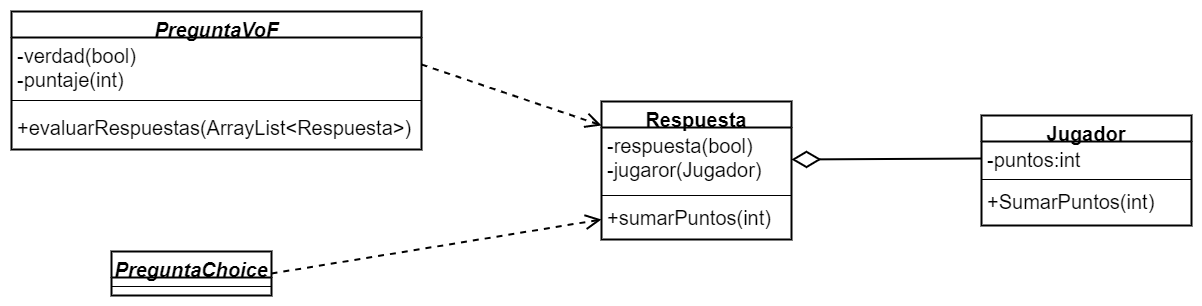
\includegraphics[width=1.3\textwidth, center]{Diagrama de clases 3.png}
\caption{\label{fig:class01}Diagrama de Clases 1.}
\end{figure}


\begin{figure}[H]
\centering
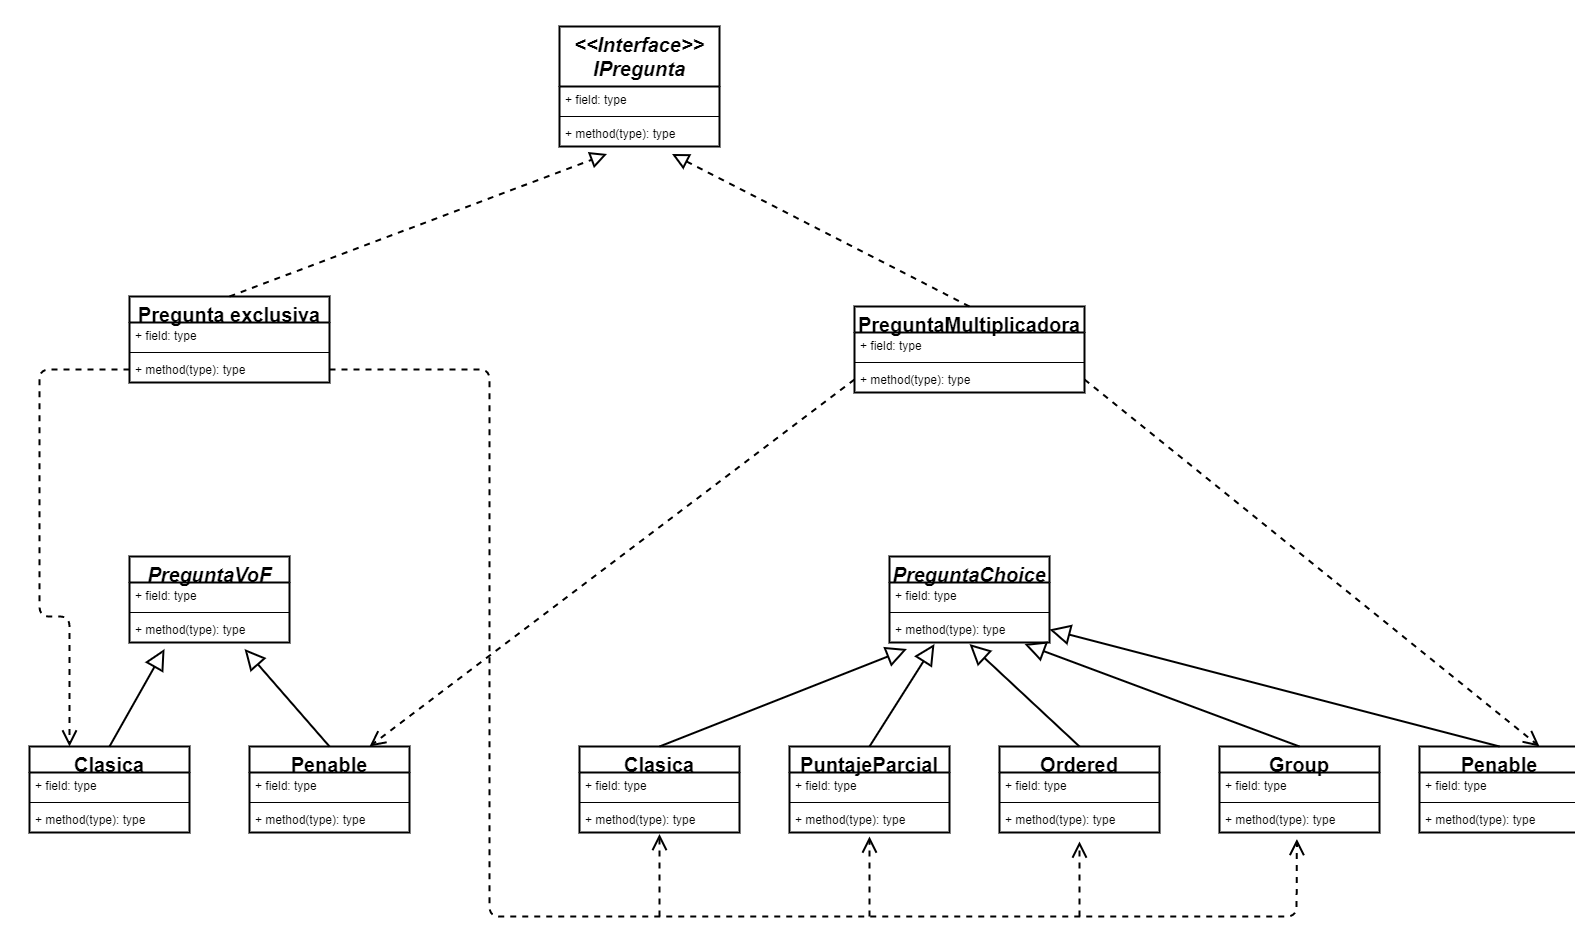
\includegraphics[width=1.3\textwidth, center]{Diagrama de clases 2.png}
\caption{\label{fig:class01}Diagrama de Clases 2.}
\end{figure}

En ellos se puede ver que existe una interfaz \textit{IPregunta} que es implementada por las clases \textit{Pregunta Exclusiva} y \textit{PreguntaMultiplicadora}, estas clases dependen de las respectivas clases de las preguntas concretas, de esta manera se plantea la implementacion de la Abstract Factory

\begin{figure}[H]
\centering
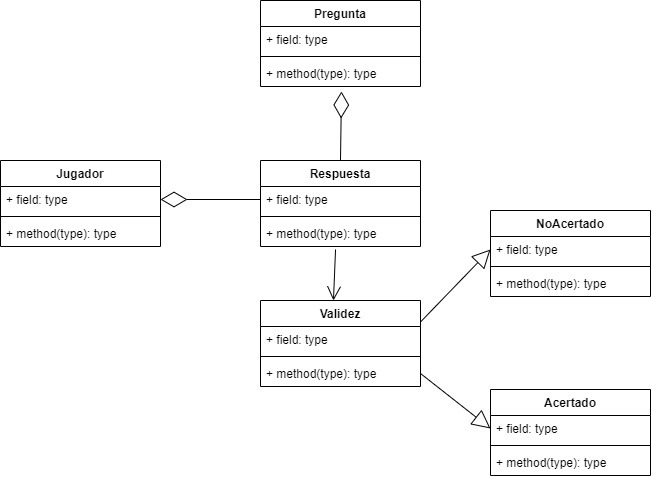
\includegraphics[width=1.3\textwidth, center]{Diagrama de clases 4.jpg}
\caption{\label{fig:class01}Diagrama de Clases 3.}
\end{figure}

Este diagrama es uno alternativo donde se plantea un modelo para eliminar la estructura \textit{if} que se encuentra en las otras clases de los demas modelos

\section{Diagramas de secuencia}\label{sec:diagramasdesecuencia}
% Mostrar las secuencias interesantes que hayan implementado. Pueden agregar texto para explicar si algo no queda claro.

\begin{figure}[H]
\centering
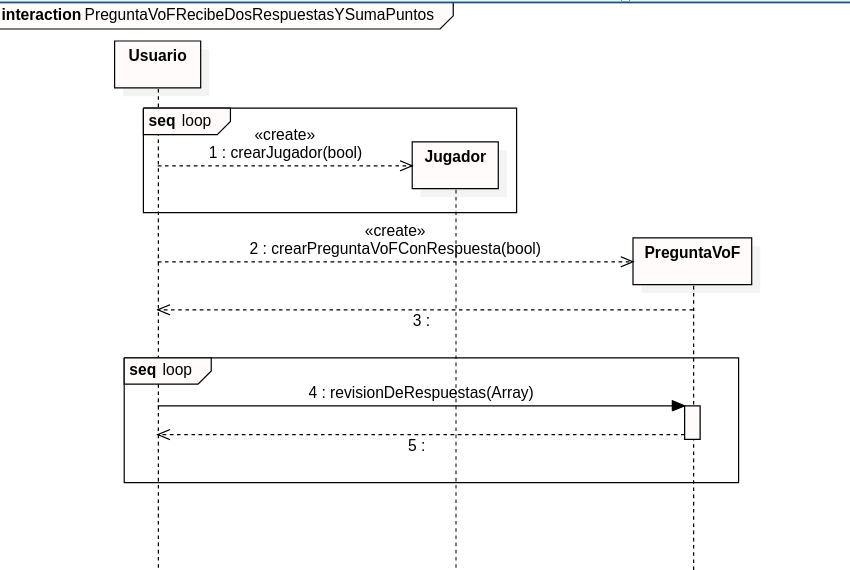
\includegraphics[width=1.35\textwidth, center]{Diagrama de secuencia.png}
\caption{\label{fig:seq01}Diagrama de secuencia 1.}
\end{figure}

Se presenta un diagrama de secuencia tentativo del caso donde una pregunta recibe una o mas respuestas y asigna los puntajes según corresponda a los jugadores que respondieron.


\section{Excepciones}\label{sec:excepciones}
% Explicación de cada una de las excepciones creadas y con qué fin fueron creadas.

\begin{description}
\item[Error1] Descripción Error 1
\item[Error2] Descripción Error 2
\end{description}

\end{document}